TODO: There should be some blabla. 

\section{Use Case Diagram}

Based on the requirements that were agreed on with the customer, two main use
cases of the system can be found:

\begin{itemize}
\item{Drive out of a perpendicular Parking Lot}
\item{Drive out of a parallel Parking Lot}
\end{itemize}

Both use cases have in common that at the end of the successful process, the
user has to regain the control over its vehicle in a defined way. Additionally,
the user should always have the possibility to interrupt the process and regain
the control over the car, even if the process has not yet finished. Each of the
use cases are triggered by the driver as well as they are supported by various
sensors and control systems.

\begin{figure}
\centering
\captionsetup{justification=centering}
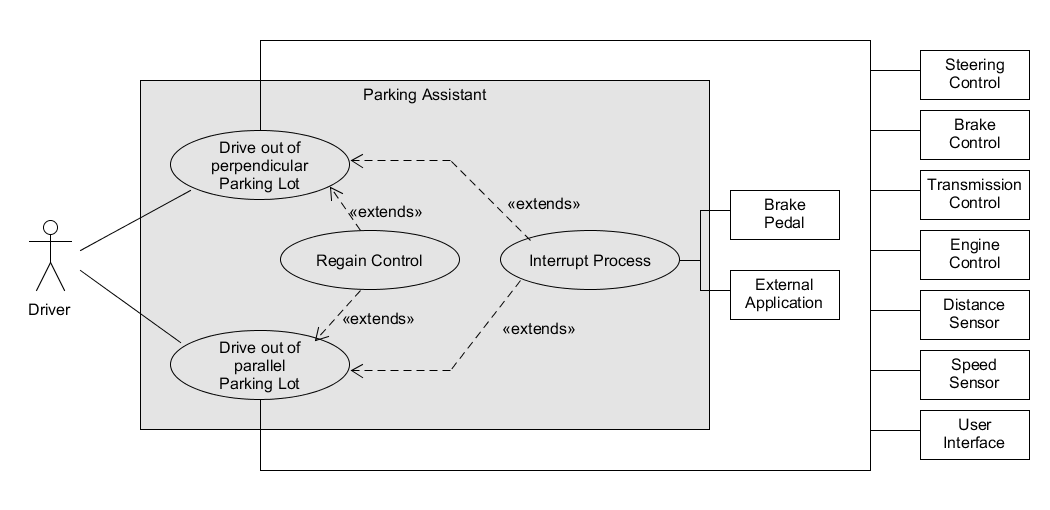
\includegraphics[width=\textwidth]{res/systemAnalysis/UseCase.png}
\caption{Overview of the System's Use Cases}
\label{fig:UseCases}
\end{figure}

\section{Sensor Overview}
To support the presented use cases, the system needs an overview of the cars
surrounding. Six sensors, two of them cameras and 4 of them distance sensors,
are placed in the car to provide this overview. The placement of the sensors can be
retrieved from figure \ref{fig:SensorOverview}.

The sensors that are placed in the middle of the car�s front and rear are
cameras. In many cases cameras are already integrated in the car and provide the
user a realistic image of its surrounding. The distance sensors at the corners
of the bumpers might be radar- or ultrasonic-sensors. Radar sensors have the
advantage, that they might be placed within the bumper and that they are
therefore not visible.

\begin{figure}
\centering
\captionsetup{justification=centering}
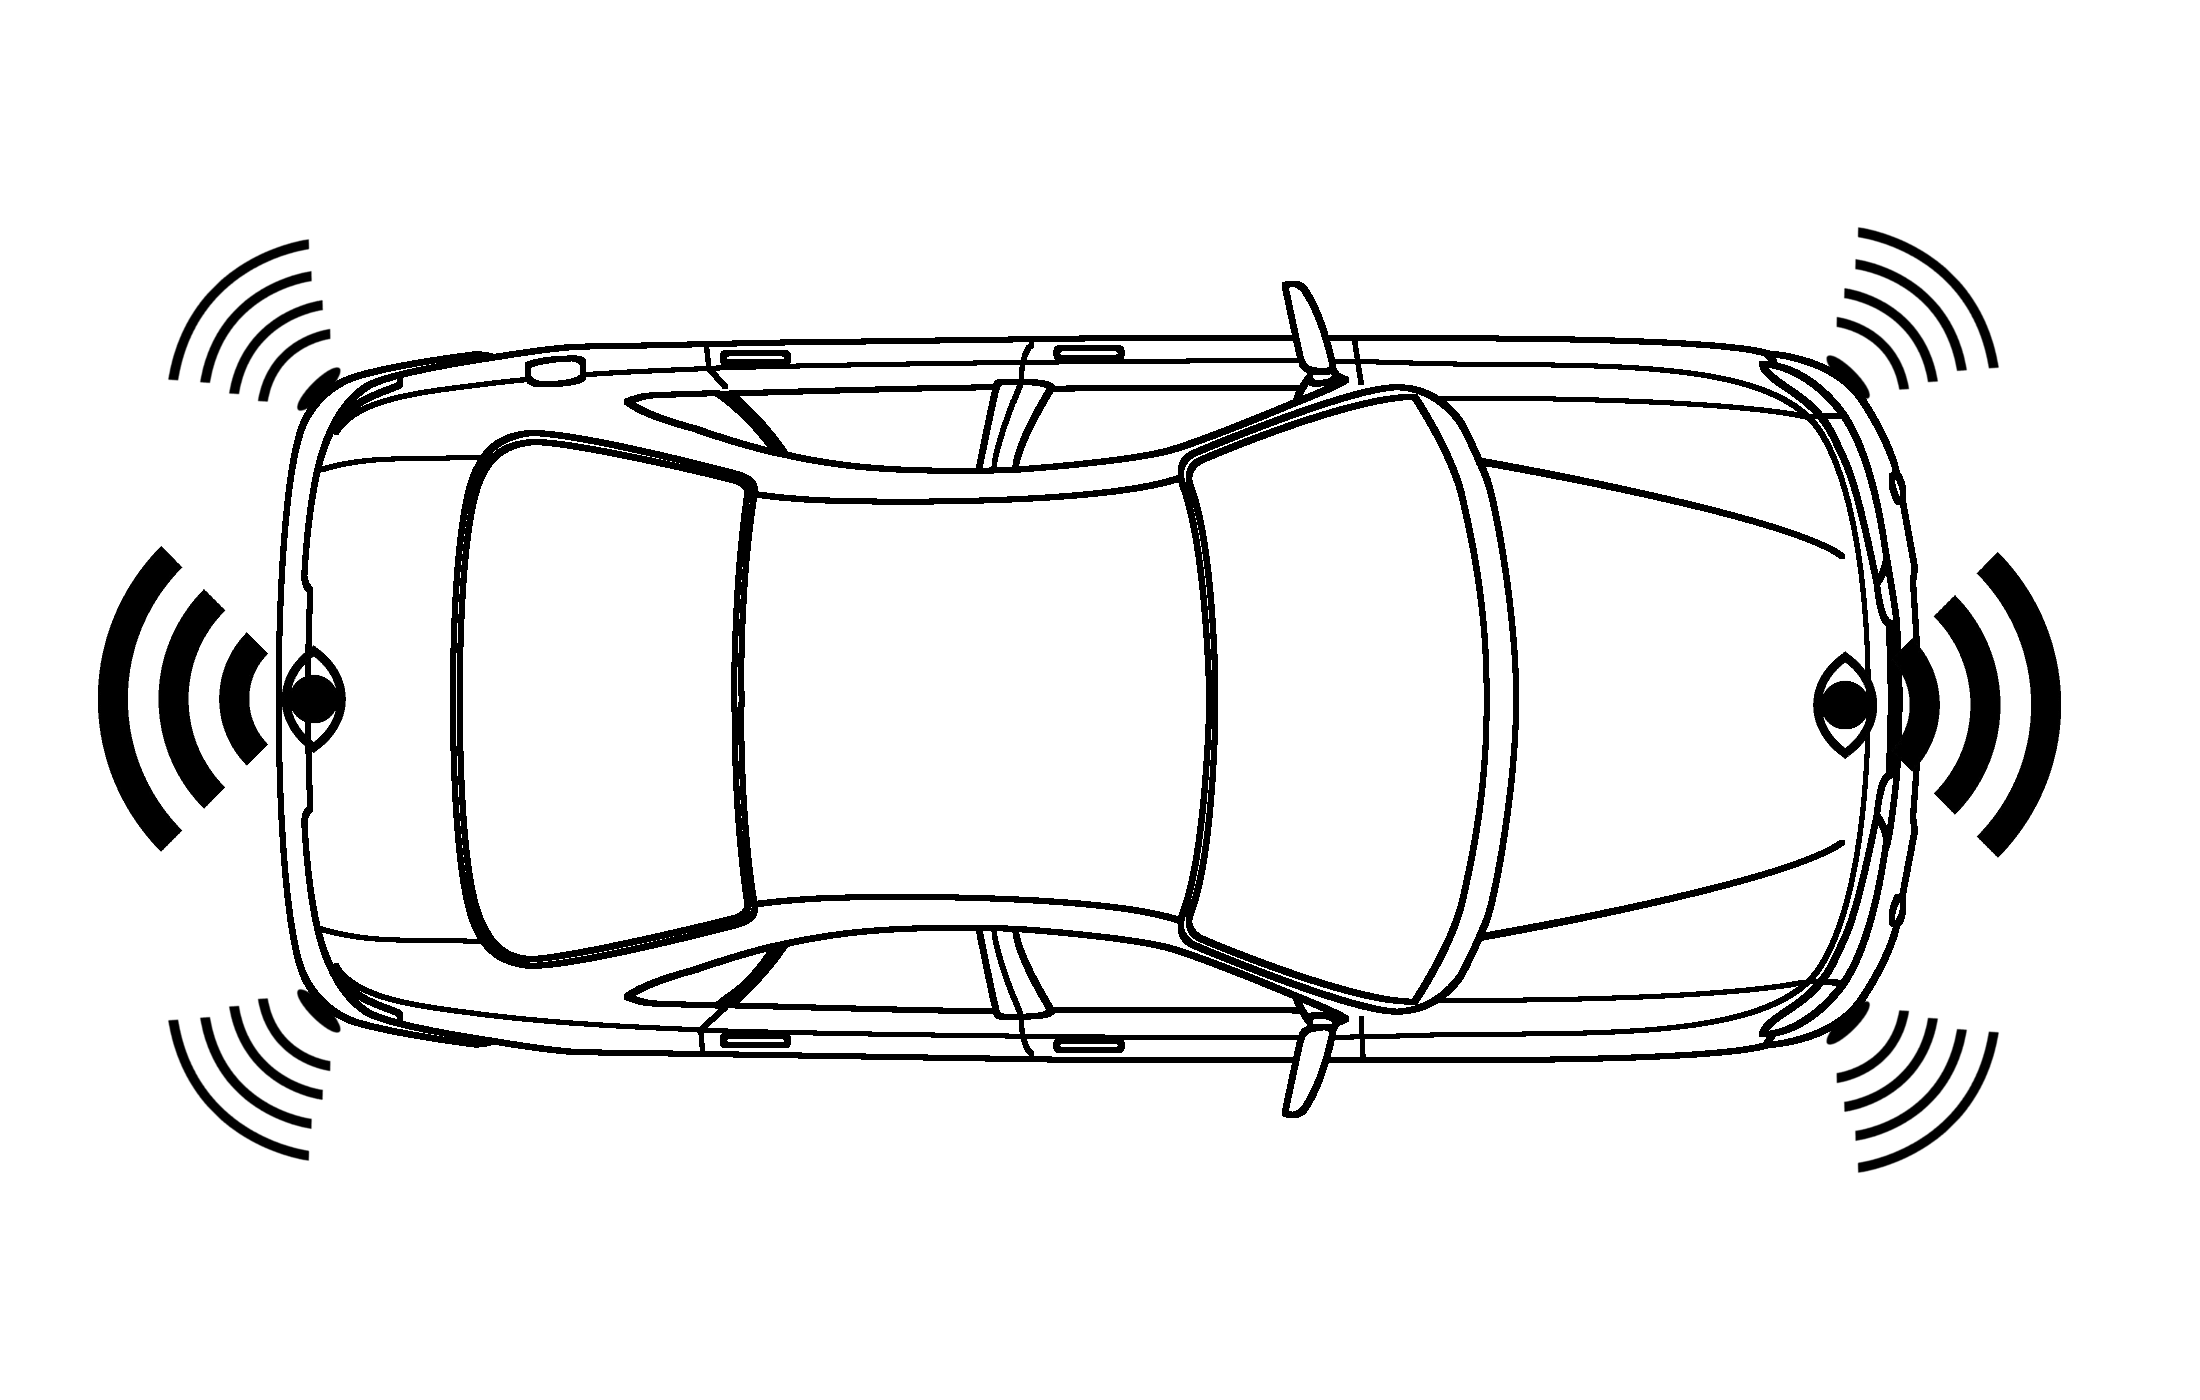
\includegraphics[width=0.75\textwidth]{res/systemAnalysis/SensorOverview.png}
\caption{Overview of the System' Sensors}
\label{fig:SensorOverview}
\end{figure}

\section{Context Diagram}

After the use cases and the required sensors have been found, the context of the
system to develop can be determined (see figure \ref{fig:ContextDiagram}).
Dataflows are depicted with solid arrows while signals that are used to control
the systems are sketched with dashed arrows.

Beside the sensor information, the graphical representation of the process and
the information that is sent to the car�s control systems, there exist two
systems that are used to interrupt the process of leaving a parking lot. If a
driver sits in the car and presses the break pedal, the process will be
interrupted immediately and the driver will regain the control over its vehicle.
If the whole process is controlled remotely without the driver sitting in its
car, the external application that controls the process should act as a dead
man�s switch that is operated by the user. If the signal from this application
is no more retrieved by the system, the process should be interrupted.


\begin{figure}
\centering
\captionsetup{justification=centering}
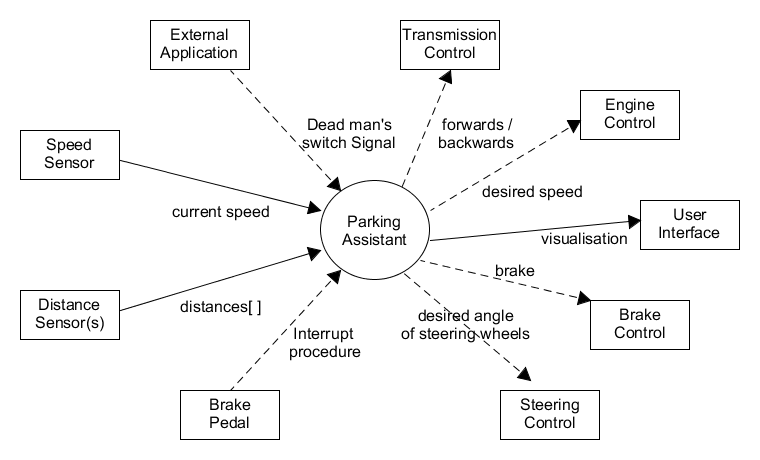
\includegraphics[width=\textwidth]{res/systemAnalysis/ContextDiagram.png}
\caption{Context Diagram of the System}
\label{fig:ContextDiagram}
\end{figure}

\section{Activity Diagrams}

Nachdem in den vorangegangen Kapiteln sowohl die Use cases als auch die
beteiligten Sensoren beschrieben wurden wird in diesem Kapitel der ablauf des
Perpendicular parking und des Parallel parking mithilfe von activity diagrammen
beschrieben. Ein activity diagram visualisiert die Dynamik und das Verhalten des
systems und tr�gt somit zu einem besseren Verst�ndnis des prozessablaufes bei. 

\subsection{Activity Diagram Reverse Perpendicular Parking}

Beim verlassen einer Perpendicular Parksituation gibt es verschiedene F�lle zu
betrachten die das System beinflussen k�nnen bzw daran hindern k�nnen gefahrlos
auszuparken. Ausserdem gibt es verschiedene Ausgangslagen, in welcher sich das
Fahrzeug befinden kann bevor der Ausparkvorgang gestartet wird. Zu diesem
Zweck wird im folgenden der Best- und der Worst Case der Ausgangslagen
beschrieben. Der Prozessablauf kann Figure \ref{fig:ActivityPerpendicular}
entnommen werden.

\begin{itemize}
\item \textbf{Best Case} \newline
Beim Best Case handelt es sich um eine Ausgangslage, bei welcher sich kein
Obstacle auf der fahrerseite des Fahrzeuges befindet. Dies wird mithilfe der
Sensoren des Fahrzeuges ermittelt. Der Gruund hierf�r ist es, dass beim
r�ckw�rtigen Ausparken das Fahrzeug direkt einlenken und zur�cksetzen kann.
Dabei ist es f�r den Reverse Perpendicular Parking Vorgang nicht von Bedeutung
ob sich ein Obstacle auf der Beifahrer seite befindent, da dies den
Ausparkvorgang nicht beeintr�chtigt. Es wird nun solange zur�ckgesetzt, bis das
Fahrzeug die Fahrbahn mithilfe der Kamera erkennt. Ausserdem wird zus�tzlich
gepr�ft, ob sich ein Fahrzeug, Fahrrad oder eine Person auf der Fahrbahn befindet. Falls dies der
Fall ist stoppt das Fahrzeug und wartet bis das Hinderniss beseitigt ist.
Befindet sich kein Hinderniss auf der Fahrbahn kann der Ausparkvorgang
fortgesetzt und beendet werden.
\item \textbf{Worst Case} \newline
Beim Schlechtfall handelt es sich um eine Ausgangslage, bei welcher fahrerseitig
ein Obstacle befindet. Dadurch ver�ndert sich der Ablauf des Prozesses, denn es
kann nun nicht mehr sofort eingelenkt werden sondern es muss zuerst
zur�ckgesetzt werden. Hierbei wird auch wieder darauf geachtet, dass sich keine
Person, Fahrrad oder Fahrzeug auf der Fahrbahn befindet. Es wird solange
zur�ckgesetzt bis fahrereseitig kein Hinderniss mehr von den Sensoren erkannt
wird. Anschlie�end kann das Fahrzeug wieder einlenken und der darauf folgende
Ablauf ist identisch, wie der beim Best Case.
\end{itemize}

\begin{figure}
\centering
\captionsetup{justification=centering}
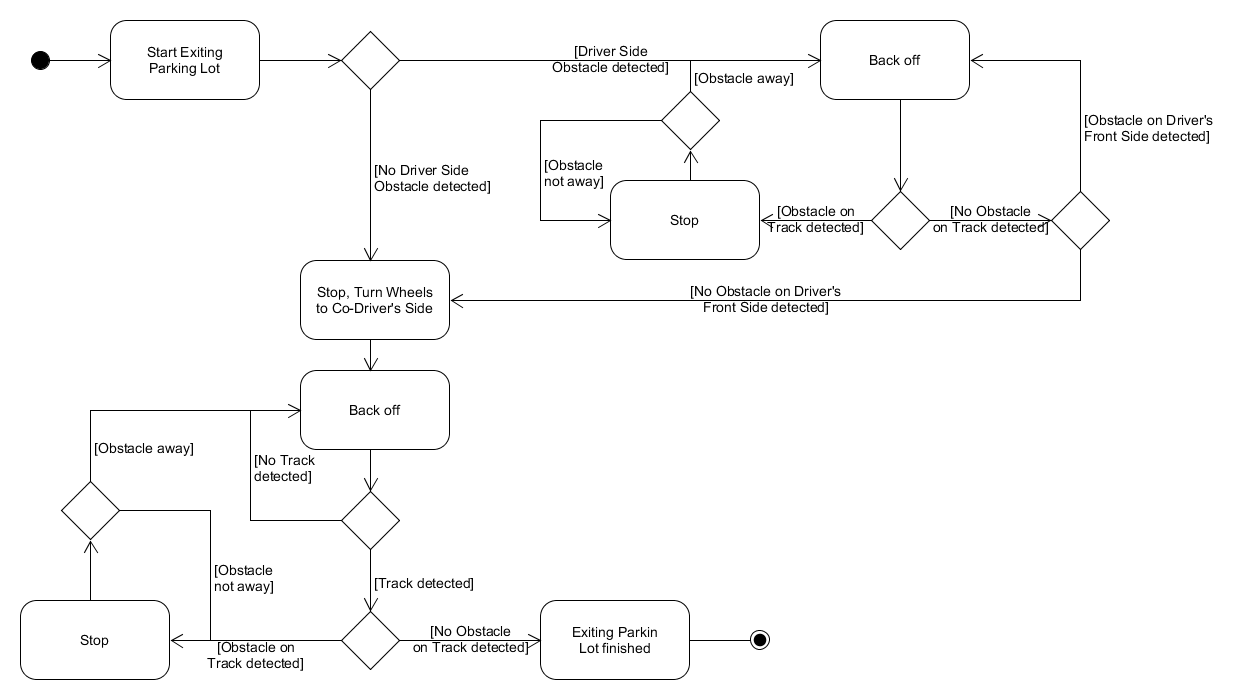
\includegraphics[width=\textwidth]{res/systemAnalysis/ActivityObstacleTransversal.png}
\caption{Algorithm for leaving a perpendicular Parking Situation}
\label{fig:ActivityPerpendicular}
\end{figure}

\subsection{Activity Diagram Parallel Parking}

Auch beim verlassen einer Parallel Parksituation gibt es wiederum verschiedene
Ausgangslagen zu betrachten, die das System beinflussen k�nnen bzw daran hindern
k�nnen gefahrlos auszuparken. Analoge zum Reverse Perpendicular Parking wird im
folgenden der Best- und der Worst Case der Ausgangslagen beschrieben. 
Der Prozessablauf kann Figure \ref{fig:ActivityParallel} entnommen werden.

\begin{itemize}
\item \textbf{Best Case} \newline
In diesem Szenario ist der Best Case der, in welchem sich kein Hinderniss vor
dem Fahrzeug befindet. Dadurch kann das Fahrzeug direkt so einlenken, dass die
Reifen weg vom Bordstein zeigen und anschlie�end Vorw�rtsfahren. Beim
Vorw�rtsfahren wird weiterhin gepr�ft, ob sich kein Hinderniss vor dem Fahrzeug
befindet. Es wird nun solange Vorw�rts gefahren, bis die Kamera die Fahrbahn
erkennt. Ausserdem wird gepr�ft, dass sich keine Hindernisse auf der Fahrbahn
befinden. Ist dies der Fall so wird der Ausparkvorgang beendet. Andernfalls
stoppt das Fahrzeug und setzt erst mit dem Ausparkvorgang fort, sobald das
Hinderniss weg ist.
\item \textbf{Worst Case} \newline
Im Schlechtfall befindet sich sowohl vor dem Fahrzeug als auch hinter dem
Fahrzeug jeweils ein Obstacle. Dies bedeutet das Fahrzeug setzt soweit zur�ck
bis es einen minimalen Abstand zum Hinderniss hat. Anschlie�end dreht es die
R�der vom Bordstein weg und f�hrt vorw�rts. Erkennt das Fahrzeug nun ein
Hinderniss vor sich, so h�lt es an, dreht seine R�der zum Bordstein hin und
f�hrt r�ckw�rts. Dies tut es wiederum solange bis es kurz vor dem r�ckw�rtigen
Hinderniss steht. Anschlie�end werden die R�der wieder vom Bordstein weggedreht
und solange vorw�rts gefahren bis die Stra�e erkennt wird. Der folgende Ablauf
des Ausparkprozesses ist wiederum identisch zum Best Case.
\end{itemize}

\begin{figure}
\centering
\captionsetup{justification=centering}
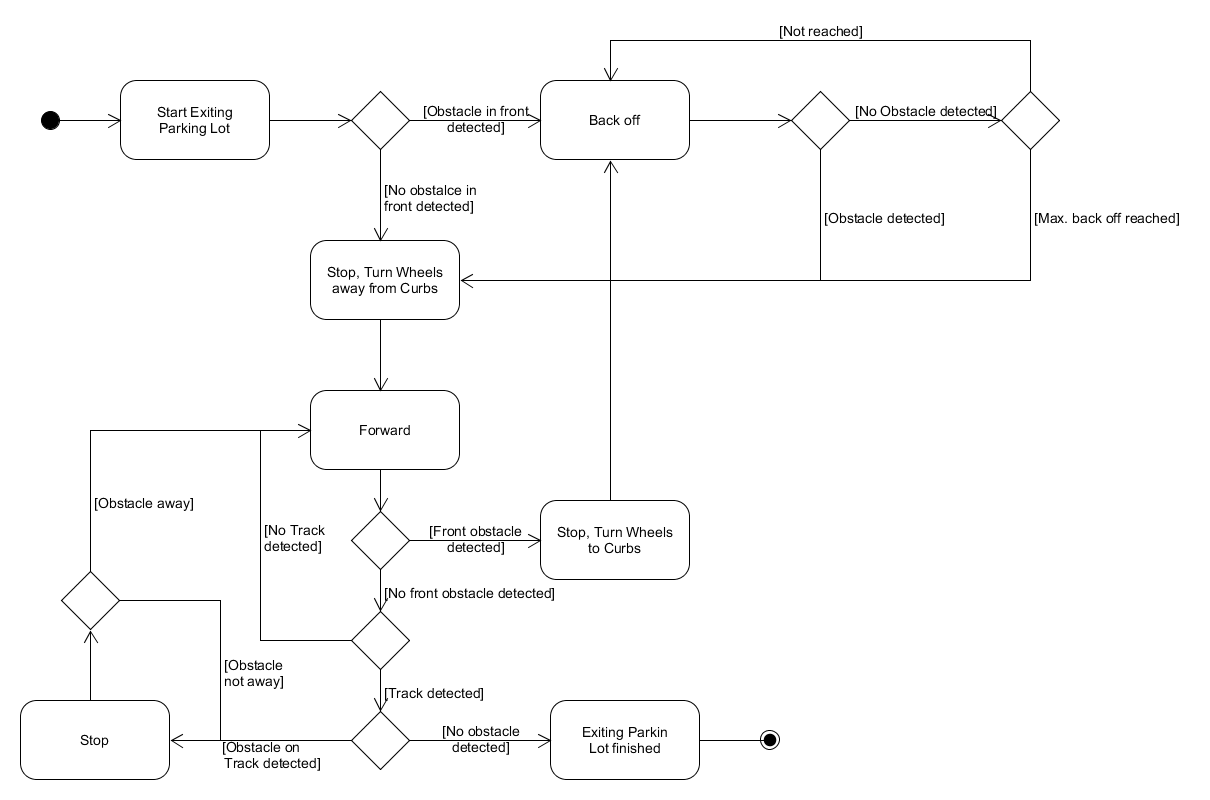
\includegraphics[width=\textwidth]{res/systemAnalysis/ActivityObstacleLenghtwise.png}
\caption{Algorithm for leaving a parallel Parking Situation}
\label{fig:ActivityParallel}
\end{figure}

\section{Design Sketches}

A first design sketch has been developed (see figure \ref{fig:initialMockup})
and the customer�s feedback on the design has been gathered, this feedback is
used to create refined mockups. Since the customer requests two designs -- one
for the day and one for the night-mode -- two of these refined designs are
developed.

These newly designed mockups also take the customer�s feedback into account that
some outputs should be simplified and that the area where the sensor information
is presented should not be reduced. Instead, the area presenting the aerial view
is reduced and the sensor information are presented in a wider area.

\begin{figure}
\centering
\captionsetup{justification=centering}
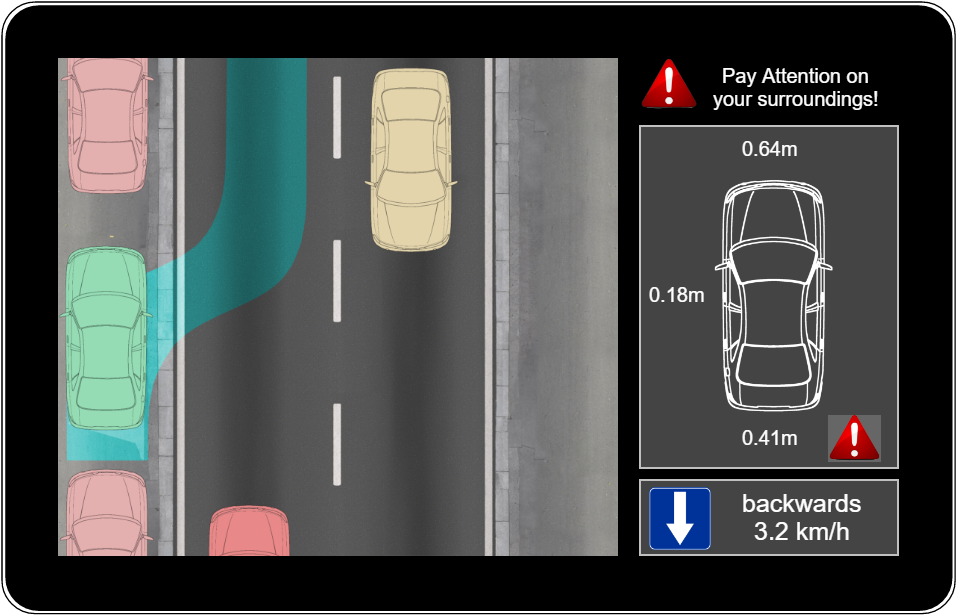
\includegraphics[width=0.75\textwidth]{res/systemAnalysis/darkskin.png}
\caption{Dark Skin of the final Design Sketch}
\label{fig:darkskin}
\end{figure}

\begin{figure}
\centering
\captionsetup{justification=centering}
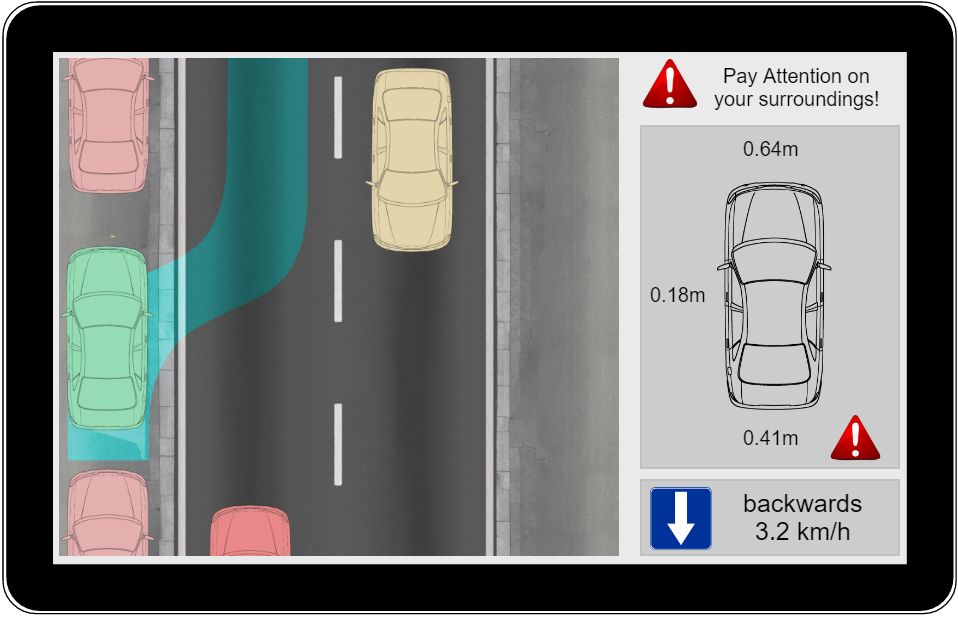
\includegraphics[width=0.75\textwidth]{res/systemAnalysis/brightskin.png}
\caption{Bright Skin of the final Design Sketch}
\label{fig:brightskin}
\end{figure}
